\documentclass{ieeeaccess}
\usepackage{cite}
\usepackage{amsmath,amssymb,amsfonts}
\usepackage{algorithmic}
\usepackage{graphicx}
\usepackage{textcomp}
\usepackage{placeins}
\usepackage{afterpage}
\usepackage{float}
\usepackage{subfig}

\def\BibTeX{{\rm B\kern-.05em{\sc i\kern-.025em b}\kern-.08em
    T\kern-.1667em\lower.7ex\hbox{E}\kern-.125emX}}
\begin{document}
\history{Date of publication xxxx 00, 0000, date of current version xxxx 00, 0000.}
\doi{10.1109/ACCESS.2017.DOI}

\title{AGENA: An Agentic AI Framework for Explainable Native Advertisement Detection in Digital News}
\author{\uppercase{Brian Rizqi Paradisiaca Darnoto\authorrefmark{1,2}, Diana Purwitasari\authorrefmark{1,*}, \IEEEmembership{Senior Member, IEEE}, Daniel Siahaan\authorrefmark{1},\IEEEmembership{Member, IEEE}
}}
\address[]{\authorrefmark{1}Informatics Department, Institut Teknologi Sepuluh Nopember, Surabaya, 60111, Indonesia}
\address[]{\authorrefmark{2}Informatics, Universitas Jember, Jember, 68121, Indonesia}

\markboth
{Darnoto \headeretal: AGENA: An Agentic AI Framework}
{Darnoto \headeretal: AGENA: An Agentic AI Framework}

\corresp{Corresponding author: Diana Purwitasari (e-mail: diana@its.ac.id)}

\begin{abstract}
Native advertising in digital news is difficult to detect because promotional intent is often embedded in factually correct editorial-style writing. Existing machine-learning and deep-learning detectors can achieve competitive classification scores, but they typically provide limited reasoning transparency for newsroom auditing. This paper proposes AGENA, an agentic framework for explainable native advertisement detection in Indonesian news. AGENA decomposes inference into five coordinated agents: Web Scraper, Preprocessing, Retriever, Classifier, and Explainer. The framework combines Retrieval-Augmented Generation (RAG) with a Reasoning-First fine-tuning strategy so that classification is grounded in retrieved evidence and accompanied by structured justification traces. Experiments on a curated corpus of 12,088 Indonesian news articles show that AGENA with Gemma 3 12B achieves 94.50\% accuracy, outperforming zero-shot and reduced-pipeline baselines. Qualitative evaluation with an LLM-as-a-Judge protocol reports a mean reasoning score of 4.4/5 and strong semantic alignment with expert annotations, indicating improved interpretability in addition to predictive performance. These results suggest that agentic, evidence-grounded LLM pipelines are a practical direction for transparent media monitoring and editorial decision support.
\end{abstract}

\begin{keywords}
Agentic AI, Explainable AI, LangChain, Native Advertising, News Classification, Retrieval-Augmented Generation.
\end{keywords}

\titlepgskip=-15pt

\maketitle

\section{Introduction}
\label{sec:introduction}
Native advertising refers to paid media content designed to resemble the editorial style of the platform on which it appears. Unlike traditional advertising formats such as banners or interstitials, native ads integrate seamlessly into news feeds and article pages, making them difficult for readers to identify as commercial content. This format raises significant concerns about editorial independence and the transparency of journalistic content \cite{b38}.

Recent marketing evidence further shows that native-ad placement and congruence strongly shape user click, bounce, and visit behavior in practice \cite{b53}. The broader media-branding literature also positions native advertising as an editorial-sponsorship boundary problem that requires explicit governance \cite{b54}.

In the Indonesian digital news landscape, native advertising is particularly prevalent. Prior Indonesian studies and datasets show that this problem is significant enough to require systematic monitoring and automated analysis \cite{b17, b21}. Automated detection of such content is therefore an important problem for media oversight.

Detecting native advertisements is inherently more complex than identifying propaganda or factual misinformation. While the latter typically relies on false claims \cite{b8}, native advertising is often factually accurate but strategically framed. Its persuasive effect stems from the selective use of promotional language: subtle hyperbole, absence of critical counterpoints, and emphasis on corporate achievements presented as news \cite{b9}. In the Indonesian context, this challenge is compounded by the diversity of regional writing styles and the use of informal idioms that complicate automated linguistic analysis. Given the dataset scale reported in prior Indonesian work, manual review is not feasible for routine monitoring \cite{b17, b19}.

Recent advances in transformer-based language models have opened new possibilities for nuanced text classification \cite{b23, b39}. However, applying these models directly to native ad detection exposes two recurring weaknesses. First, standard LLMs often produce labels without transparent, auditable reasoning, limiting their utility in newsroom workflows. Second, they can hallucinate when domain grounding is weak; retrieval-augmented generation (RAG) mitigates this by conditioning inference on retrieved evidence \cite{b25}. A framework that combines the reasoning capacity of LLMs with domain grounding and interpretable outputs is therefore needed.

In addition, recent retrieval research in advertising and sponsored-search contexts indicates that real-time, intent-aware retrieval design is increasingly important when language models are deployed in production decision pipelines \cite{b22}.

Recent NLP pipelines increasingly rely on large pretrained transformers and scaling principles for low-resource adaptation \cite{b15, b39}. In journalism-oriented settings, robustness and hallucination risks remain central concerns for trustworthy deployment \cite{b50, b55}.

Prior work on automated native ad detection, including the SENADA framework, relied on stacked ensemble classifiers that decompose the detection task into independent sub-models for sentiment, persuasion, promotion, and perspective \cite{b17, b19}. These approaches established strong performance benchmarks, but they lack interpretability and cannot generate justifications that editors can review. This is a significant limitation in practice, as editorial oversight requires not just a decision, but an explanation of why a piece of content was flagged. This interpretability gap has also been discussed in prior Indonesian studies on persuasive content detection in electronic news \cite{b21}.

This paper introduces AGENA (Agentic AI Framework for Explainable Native Advertisement Detection), a multi-agent system that addresses these gaps. AGENA decomposes the detection task into a sequential pipeline of five specialized agents: (1) a Web Scraper for content extraction, (2) a Preprocessor for linguistic feature engineering, (3) a Retriever for RAG-based context grounding, (4) a Classifier for chain-of-thought reasoning, and (5) an Explainer for generating auditable justifications.

The main contributions of this work are:
\begin{enumerate}
    \item \textbf{Architectural contribution}: We propose the AGENA pipeline, a five-agent system for native advertisement detection in Indonesian digital news. To our knowledge, this is the first dedicated multi-agent detection framework for this domain.
    \item \textbf{Methodological contribution}: We introduce a ``Reasoning-First'' fine-tuning strategy grounded in RAG, anchored to a curated knowledge base of 12,088 Indonesian news articles. This approach reduces hallucination and improves discrimination of ``Ambiguous'' cases.
    \item \textbf{Evaluative contribution}: We evaluate model output quality beyond accuracy metrics using an ``LLM-as-a-Judge'' protocol, in which GPT-4o rates reasoning traces on a 1--5 scale across four interpretability criteria: Sentiment, Persuasion, Promotion, and Perspective alignment.
\end{enumerate}

The remainder of this paper is organized as follows. Section II surveys related work across machine learning, LLMs, and agentic AI for media analysis. Section III describes the dataset. Section IV presents the AGENA architecture and algorithms. Section V reports experimental results. Sections VI and VII discuss implications and conclusions.

\section{Related Works}
\label{sec:related-works}
We discuss prior work across three areas relevant to AGENA: machine learning for advertisement detection, large language models with retrieval augmentation, and agentic AI systems.

\subsection{Machine Learning and Deep Learning in Ad Detection}
Early approaches to automated native ad detection in Indonesian news relied on lexical and statistical features combined with conventional classifiers, providing useful baselines but limited linguistic depth \cite{b18, b21}.

Deep learning approaches improved upon this by enabling automatic feature extraction and richer semantic modeling in Indonesian native ad detection \cite{b18, b19}. A notable system in this space is SENADA, which decomposed the detection task into four ensemble sub-models aligned with the theoretical dimensions of persuasion (Sentiment, Persuasion, Promotion, Perspective) \cite{b19}. Despite strong results, these models lacked explanatory output, limiting their adoption in editorial settings where decision transparency is required.

Beyond Indonesian datasets, recent benchmark and survey studies in fake-news detection also highlight reproducibility, feature diversity, and early-detection constraints as recurring methodological issues \cite{b52, b55}.

Foundational social-media fake-news surveys further emphasize the importance of combining content signals with propagation context and source credibility \cite{b60, b62}. Additional evidence from rumor-oriented studies also supports using user-level behavioral cues for credibility assessment \cite{b61, b66}.

\subsection{Large Language Models and Retrieval-Augmented Generation}
The Transformer architecture \cite{b23} established a new baseline for text classification tasks. BERT and related transformer models have substantially improved contextual language modeling and downstream classification performance \cite{b39}. In the news domain, these advances support finer-grained analysis of framing and persuasive signals \cite{b8, b9}.

A recurring limitation of standalone LLMs is domain-specific hallucination. Retrieval-Augmented Generation (RAG) addresses this by coupling an inference model with a vector database, enabling it to retrieve and condition on relevant prior examples \cite{b25}. This design is particularly useful for news monitoring tasks, where retrieved historical examples can serve as grounding evidence for classifying new articles. Most existing RAG systems, however, operate as single-step retrieval pipelines and do not support multi-step, autonomous decision-making.

Recent fake-news detection research also reports that social-context modeling can substantially improve discrimination for hard content-only cases \cite{b67}.

Recent large-scale reviews similarly emphasize that explainability and robustness remain unresolved in modern misinformation pipelines \cite{b50, b57}.

At the systems level, operational RAG stacks require robust retrieval quality control, reproducible evaluation protocols, and reliable indexing workflows \cite{b52, b57}.

In parallel, ensemble-oriented architectures in high-volume settings continue to report competitive performance for deceptive-content screening workflows \cite{b52}.

\subsection{Emergence of Agentic AI and Multi-Agent Systems}
In this study, agentic AI refers to systems in which LLMs function as autonomous reasoning engines, capable of planning, tool use, and multi-step execution.

Recent survey work reports increasing interest in agentic approaches for complex text analytics tasks \cite{b10}.

Agentic systems are particularly relevant to tasks requiring iterative retrieval, verification, and explanation under constrained evidence. For Indonesian digital journalism specifically, agentic approaches are well-suited, as they can incorporate language-specific tools and region-specific knowledge bases that generic classifiers would not capture. The inclusion of a dedicated Explanation Agent also addresses the interpretability requirement highlighted in prior Indonesian studies on persuasive news analysis \cite{b21}. AGENA extends this line of work by providing a dedicated multi-agent pipeline for native advertisement detection in Indonesian news, with an emphasis on classification accuracy and reasoning transparency.

This emphasis on traceable reasoning is consistent with broader explainable-AI guidance in both survey and taxonomy literature \cite{b49, b51}.

Practical black-box explanation methods are commonly operationalized through local surrogate explanations and additive attribution frameworks \cite{b64, b63}.

Foundational interpretability references in the Springer literature also reinforce this requirement for inspectable decision pipelines \cite{b59}.

Recent journalism-focused XAI reviews further stress that editorial deployment benefits from transparent and contestable model outputs, particularly for high-impact moderation contexts \cite{b20}. Broader comparative analyses also discuss model-specific behavioral bias in large language models, reinforcing the need for architecture-aware evaluation \cite{b24}. At the engineering level, parameter-efficient adaptation and attention-acceleration methods remain central for practical LLM deployment, including LoRA and FlashAttention-style optimization \cite{b36, b37}. Prior local framework studies additionally illustrate the value of implementation-efficient pipeline design in Indonesian research settings \cite{b48}. Finally, evidence from large-scale diffusion studies indicates that false information can propagate faster than verified content, motivating robust detection and explanation pipelines for public information ecosystems \cite{b65}.

\section{Dataset and Annotation}
\label{sec:dataset}
The foundation of this study is an extensive dataset of Indonesian-language electronic news articles, specifically curated for native advertisement detection \cite{b17}. The dataset comprises 12,088 articles collected from six major Indonesian news portals (e.g., Kompas, Detik, Tempo) between February and August 2022. This collection covers diverse categories as summarized in Table \ref{tab:dataset_stats}.

\begin{table}[htbp]
\caption{Dataset Distribution across News Categories}
\label{tab:dataset_stats}
\begin{center}
\begin{tabular}{|l|c|c|c|}
\hline
\textbf{Category} & \textbf{Total Articles} & \textbf{Native Ads} & \textbf{Pure News} \\
\hline
Economy & 1,914 & 1,349 & 565 \\
Lifestyle & 1,807 & 415 & 1,392 \\
Entertainment & 635 & 128 & 507 \\
International & 359 & 90 & 269 \\
National & 1,262 & 595 & 667 \\
Others & 3,565 & 2,882 & 683 \\
Automotive & 474 & 106 & 368 \\
Education & 274 & 70 & 204 \\
Sports & 823 & 69 & 754 \\
Technology & 975 & 340 & 635 \\
\hline
\textbf{Total} & \textbf{12,088} & \textbf{5,944} & \textbf{6,144} \\
\hline
\end{tabular}
\end{center}
\end{table}

A critical aspect of this dataset is its multi-label annotation. Each article was manually annotated by three independent experts based on four implicit characteristics: (1) positive or neutral sentiment, (2) persuasive tone, (3) promotional focus, and (4) single-source perspective. The inter-annotator agreement, measured via Fleiss' Kappa, reached 0.90, indicating high reliability. In AGENA, this dataset serves a dual purpose: it was used for fine-tuning the underlying Large Language Models (LLMs) and acts as the ground-truth knowledge base for the Retrieval-Augmented Generation (RAG) component, stored in a high-dimensional vector space for real-time context retrieval.

\section{Proposed Method}
\label{sec:methods}
The AGENA framework (Agentic Native Ads detection) is conceptualized as a distributed multi-agent system that shifts the detection paradigm from a singular classification event to a multi-stage collaborative reasoning process. The architecture is grounded in the "Reasoning-First" principle, where the generation of interpretative evidence is treated as an essential precursor to the final classification label.

\subsection{Philosophical Foundation: Reasoning-First Paradigm}
Traditional news classifiers operate as discriminative models that map an input $X$ directly to a label $Y$. While efficient, this approach provides no insight into the linguistic "why" behind a decision. AGENA adopts a generative-reasoning approach where the model must first construct a multi-dimensional reasoning trace $T$. This trace acts as a semantic bridge, mapping the article's features back to the theoretical characteristics of native advertising. By forcing the model to articulate its findings before committing to a label, we significantly mitigate the risk of stochastic hallucinations and improve the precision of the classification.

\subsection{Formal Definition and State Management}
We define the AGENA system not as a linear trajectory, but as a dynamic, cyclic state-transition system driven by a LangChain \texttt{StateGraph}. Let $S_{state}$ be a global state dictionary that acts as the memory buffer for the entire detection pipeline. The state space is defined by the following schema:
\begin{equation}
S_{state} = \{U, D, F, K, R\}
\end{equation}
where $U$ represents the target URL, $D$ is the extracted raw document text, $F$ is a vector of syntactic and semantic features, $K$ is the retrieved augmented context, and $R$ is the final reasoning result containing the Boolean prediction and the explanation trace.

The detection task is decomposed into five cooperative agents $A = \{A_{scrape}, A_{prep}, A_{ret}, A_{class}, A_{exp}\}$. These are separated into two subgroups: deterministic non-AI agents ($A_{scrape}, A_{prep}$) responsible for data preparation, and AI-based agents ($A_{class}, A_{exp}$) with RAG support ($A_{ret}$) for decision-making:
\begin{itemize}
    \item \textbf{Scraper Agent ($A_{scrape}$, Non-AI)}: Executes a state mutation $\delta_{scrape}: S_{state}[U] \rightarrow S_{state}[D]$. It is purely rule-based and extracts dynamic DOM nodes via a headless browser before writing the cleaned HTML $D$ to the buffer. No AI models are used in this loading phase.
    \item \textbf{Preprocessing Agent ($A_{prep}$, Non-AI)}: Executes $\delta_{prep}: S_{state}[D] \rightarrow S_{state}[F]$. This deterministic programming agent processes $D$ to extract $n$-dimensional linguistic features (e.g., word density, capitalization ratio) utilizing Regex. Similarly to the Scraper, this stage does not rely on the execution of any language model.
    \item \textbf{Retriever Agent ($A_{ret}$)}: This intermediary inference agent utilizes the \texttt{VectorSearchTool} to compute semantic proximity against a FAISS database to anchor the classification model's claims.
    \item \textbf{Classifier Agent ($A_{class}$, AI-Based)}: Implements the core neural evaluative logic $\delta_{class}: (S_{state}[D], S_{state}[F], S_{state}[K]) \rightarrow L$, where $L \in \{0, 1\}$. It leverages a fine-tuned foundation LLM to reach a Boolean decision.
    \item \textbf{Explanation Agent ($A_{exp}$, AI-Based)}: Executes the post-hoc mutation $\delta_{exp}: (S_{state}[D], S_{state}[K], L) \rightarrow S_{state}[R]$. This independent LLM agent is tasked with providing rationalization for the Classifier agent's choices through original text tracing.
\end{itemize}

\subsection{Hierarchical Agentic Orchestration}
Unlike traditional linear pipelines, the interaction between agents in AGENA is governed by a stateful graph. The orchestrator manages an "Agentic Context Buffer" that accumulates info gradients from each node.
Figure~\ref{fig:agena_toolsets} presents the complete orchestration view, including inter-agent dependencies, state mutations, and the decision checkpoints used to produce the final label and explanation.


\subsection{Detailed Agent Toolsets and Decision Logic}
Each agent within the AGENA ecosystem is equipped with specialized toolsets:

\begin{figure*}[t]
\centering
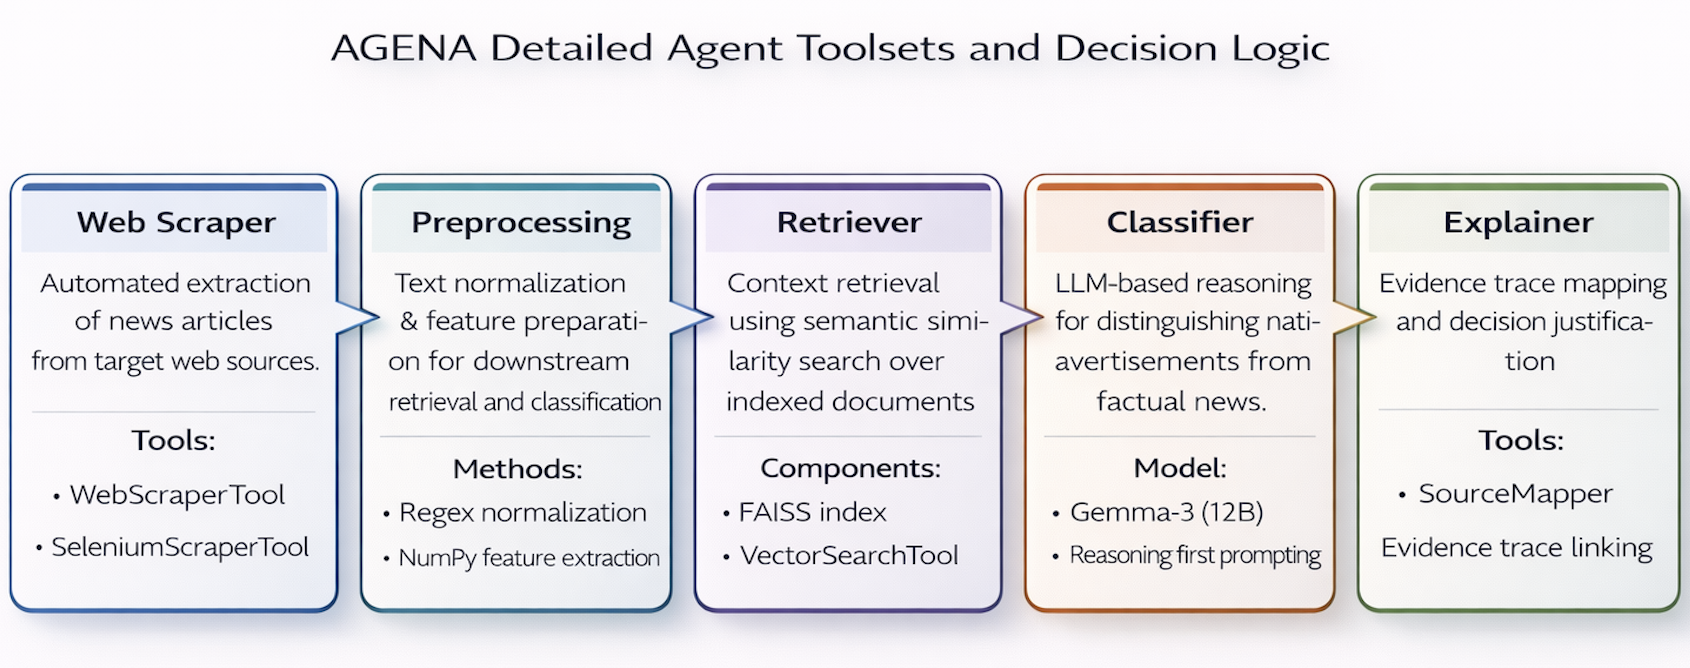
\includegraphics[width=0.98\textwidth]{agena_toolsets_flow.png}
\caption{AGENA toolsets and decision flow across the five-agent pipeline.}
\label{fig:agena_toolsets}
\end{figure*}

As shown in Figure~\ref{fig:agena_toolsets}, the pipeline starts from URL ingestion and proceeds through five tightly coupled phases. In the first phase, the Scraper Agent performs robust content acquisition from heterogeneous portal layouts and dynamic page elements. In the second phase, the Preprocessing Agent transforms raw article text into normalized linguistic representations and handcrafted indicators (e.g., lexical density, capitalization ratio, and persuasive cue markers) to make downstream reasoning more stable. In the third phase, the Retriever Agent queries the FAISS-backed memory bank to fetch semantically similar historical examples that function as evidence anchors for current inference.

The fourth phase is the Classifier Agent, which integrates three evidence streams (raw narrative content, engineered features, and retrieved context) under constrained prompting to produce a label with an explicit reasoning trace. The fifth phase is the Explanation Agent, which maps abstract reasoning claims back to concrete text spans so that each prediction can be audited by editors. The orchestration layer also enforces state consistency between phases, preventing missing-context decisions and reducing hallucination risk by requiring evidence availability before final classification. This design is central to AGENA's objective of combining competitive predictive performance with operational transparency.

\subsubsection{Web Scraper Agent (Non-AI)}
This deterministic preliminary agent utilizes the \texttt{Web\allowbreak Scraper\allowbreak Tool} and \texttt{Selenium\allowbreak Scraper\allowbreak Tool} toolsets, combining \texttt{Beautiful\allowbreak Soup4} for static DOM interfaces and \texttt{Selenium} for dynamic HTML content. It is tasked with stripping the page's text hierarchy (preprocessing cleaning), removing non-journalistic entities (e.g., footer elements, third-party ad inserts). This stage operates entirely on classic algorithmic scripts without predictive model intervention (non-AI).

\subsubsection{Preprocessing Agent (Non-AI)}
Similar to the Scraper framework, the preprocessing step exclusively uses standard deterministic engineering algorithms (non-AI):
\begin{enumerate}
    \item \textbf{Text Normalization}: Regex algorithms are used to detect the semantic hierarchy of the article, removing spatial redundancy phrases and dangling URLs.
    \item \textbf{Feature Extraction}: Compiles syntactic lexicon libraries and \texttt{numpy} array calculations for text length density variables, unique phrase percentages, and capitalization ratio coefficients in a programmatically statistical manner without deep NLP inference.
\end{enumerate}

\subsubsection{Retriever Agent}
The Retriever Agent implements semantic retrieval using a FAISS (Facebook AI Similarity Search) index backed by sentence embeddings generated with \texttt{sentence\allowbreak-transformers/all\allowbreak-MiniLM\allowbreak-L6\allowbreak-v2}. For a given input article, the agent queries the FAISS index via a \texttt{VectorSearch\allowbreak Tool}, which calls \texttt{similarity\allowbreak\_search\allowbreak\_with\allowbreak\_score} to retrieve the top-$k$ nearest neighbors from the 12,088-article knowledge base. These retrieved examples serve as in-context grounding evidence for the Classifier Agent. The retrieval process is formalized in Algorithm 1.

\subsubsection{Classifier Agent}
This agent is the core reasoning component of the pipeline. In the experiments reported here, it is built upon Gemma 3 (12B), fine-tuned on the Indonesian native advertisement dataset using the Reasoning-First strategy described in Section~\ref{sec:methods}. The agent's decision boundary is shaped by a hierarchical prompt that includes a persona layer (defining the agent as a senior news editor), a domain layer encoding Indonesian editorial standards, and a constraint layer that enforces a structured JSON output schema for downstream parsing.

\subsubsection{Explanation Agent}
This agent operates as a post-processor for the LLM output. It utilizes a \texttt{Source\allowbreak Mapper} tool to link specific reasoning claims back to original text snippets. For example, if the Classifier identifies "Excessive brand mention," the Explanation Agent scans the text to provide the exact frequency and locations of that brand name, providing empirical verification for the model's claim.

\subsection{Algorithmic Depth}
The core operational logic for the RAG-grounded reasoning is presented in Algorithm 1, while the specialized "Reasoning-First" alignment strategy is defined in Algorithm 2.

\begin{algorithmic}
\STATE \textbf{Algorithm 1: Agentic Classification with RAG}
\REQUIRE Raw Article $D$, Vector KB $K$
\ENSURE Classification Label $L$, Reasoning Trace $T$
\STATE $D^* \leftarrow S.Extract(D)$ \COMMENT{High-fidelity extraction}
\STATE $F \leftarrow P.distill(D^*)$ \COMMENT{Syntactic feature engineering}
\STATE $Context \leftarrow R.search(D^*, K, k=5)$ \COMMENT{Semantic anchoring}
\STATE $T, L \leftarrow C.reason(D^*, F, Context)$ \COMMENT{Reasoning-First execution}
\RETURN $L, T$
\end{algorithmic}

\begin{algorithmic}
\STATE \textbf{Algorithm 2: Reasoning-First Prompt Alignment}
\REQUIRE Input $X$, Characteristics $C_{markers}$, Examples $E_{shots}$
\ENSURE Aligned Trace $T$
\STATE Define System Identity $I \leftarrow \text{"Senior News Editor"}$
\FOR{each $m \in C_{markers}$}
    \STATE $Step_m \leftarrow \text{Analyze } X \text{ for characteristic } m$
\ENDFOR
\STATE $Context \leftarrow \text{Aggregate } (Step_m)$
\STATE $T \leftarrow \text{SynthesizeContext}(I, Context, E_{shots})$
\RETURN $T$
\end{algorithmic}

\subsection{Prompt Engineering and Few-Shot Alignment}
To minimize hallucinations and improve classification accuracy, AGENA employs a ``Reasoning-First'' prompting strategy. Unlike standard zero-shot classification, the Classifier Agent is instructed to perform a chain-of-thought analysis before outputting the final label. The prompt structure is defined as follows:

\begin{itemize}
    \item \textbf{System Identity}: Defines the agent as a senior editor with expertise in detecting hidden commercial intent.
    \item \textbf{Characteristic Anchoring}: Forces the agent to evaluate the text against the four theoretical markers (Sentiment, Persuasion, Promotion, Perspective).
    \item \textbf{Contextual Injection}: Injects the top-5 most similar retrieved articles to serve as semantic boundary markers.
    \item \textbf{Response Constraints}: Enforces a specific JSON schema to facilitate programmatic parsing and downstream explanation mapping.
\end{itemize}

The core reasoning engines (Qwen, Gemma, Llama, and GPT-4o) utilized in the AGENA framework are optimized for specific roles. Each model serves a distinct purpose, either as the primary classifier agent or as the evaluation judge.


An example of the few-shot template used during the fine-tuning of the Gemma 3 12B model is provided in the supplemental materials. This template teaches the model to distinguish ``positive reporting'' from ``promotional bias'' through structured reasoning steps.

\subsection{Model Tuning and Hyperparameters}
The core reasoning engines (Qwen, Gemma, Llama) were fine-tuned using Parameter-Efficient Fine-Tuning (PEFT) techniques, specifically Low-Rank Adaptation (LoRA) and 4-bit quantization (QLoRA). This approach allowed for the optimization of large-scale models within the constraints of available GPU memory. The hyperparameters used for fine-tuning are detailed in Table \ref{tab:hyperparameters}.

\subsection{Backbone Architecture Comparison}
To make model-level differences explicit, Figure~\ref{fig:model_architectures} presents the four backbone architectures evaluated in this study: Gemma 3 12B, Qwen 14B, Llama 3.1 8B, and GPT-OSS 20B. These architecture cards summarize each model's structural profile, context handling capacity, and deployment-oriented efficiency characteristics.

\begin{figure*}[t]
\centering
\subfloat[Gemma 3 12B]{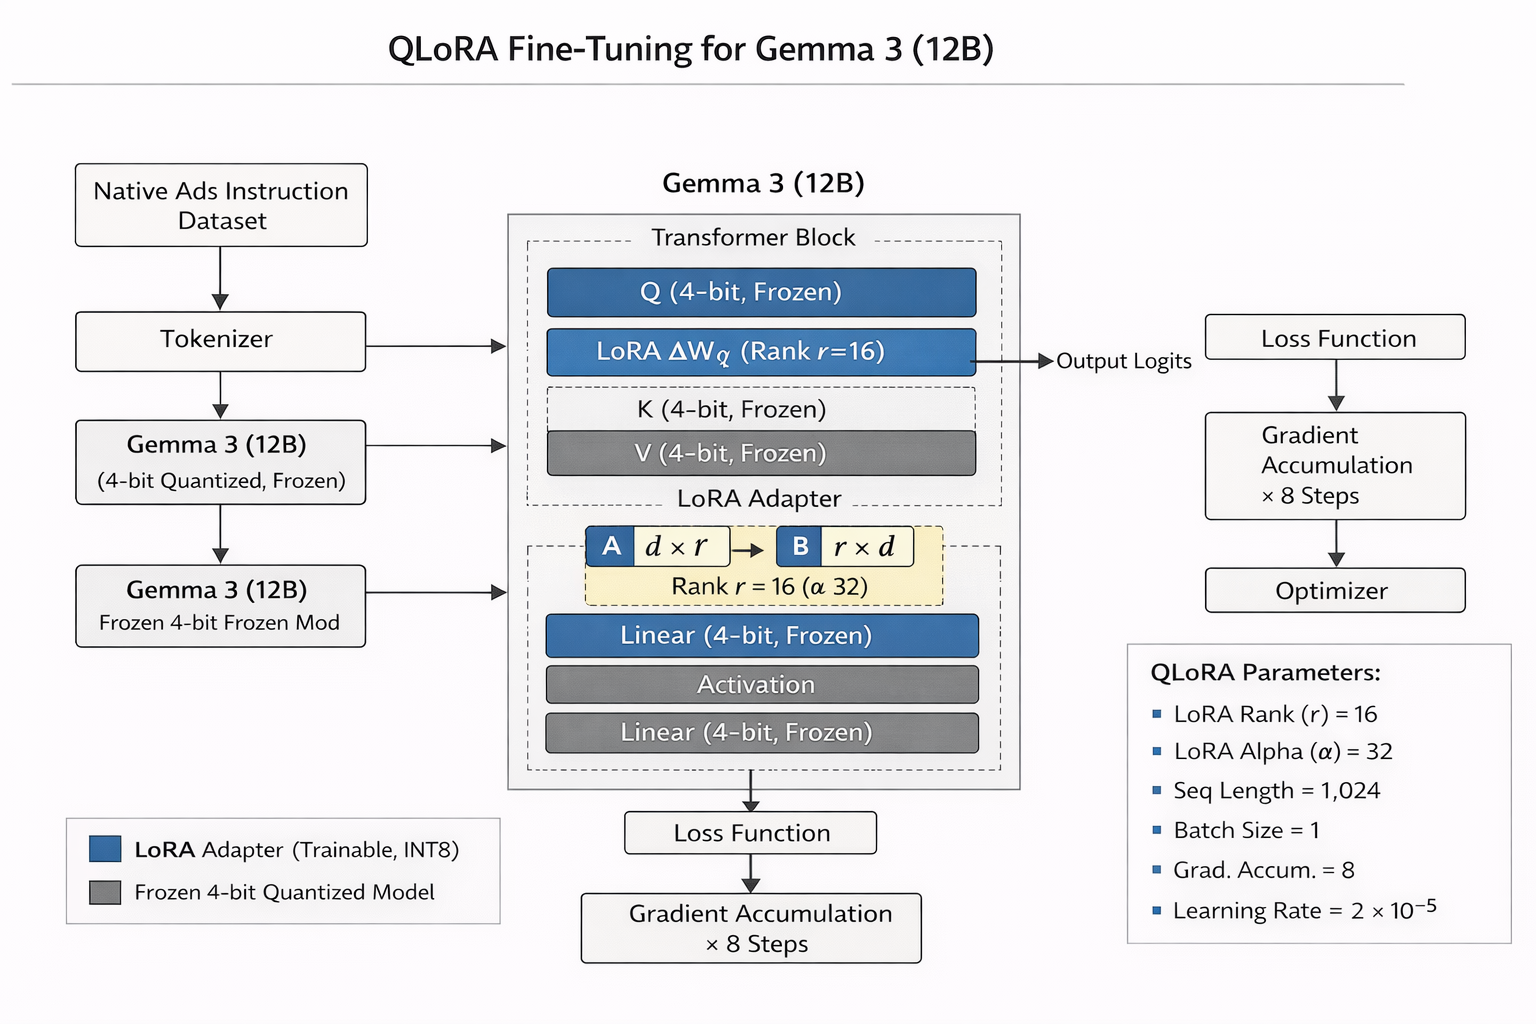
\includegraphics[width=0.46\textwidth]{architectures/gemma_3_12b.png}\label{fig:arch_gemma}}
\hfill
\subfloat[Qwen 14B]{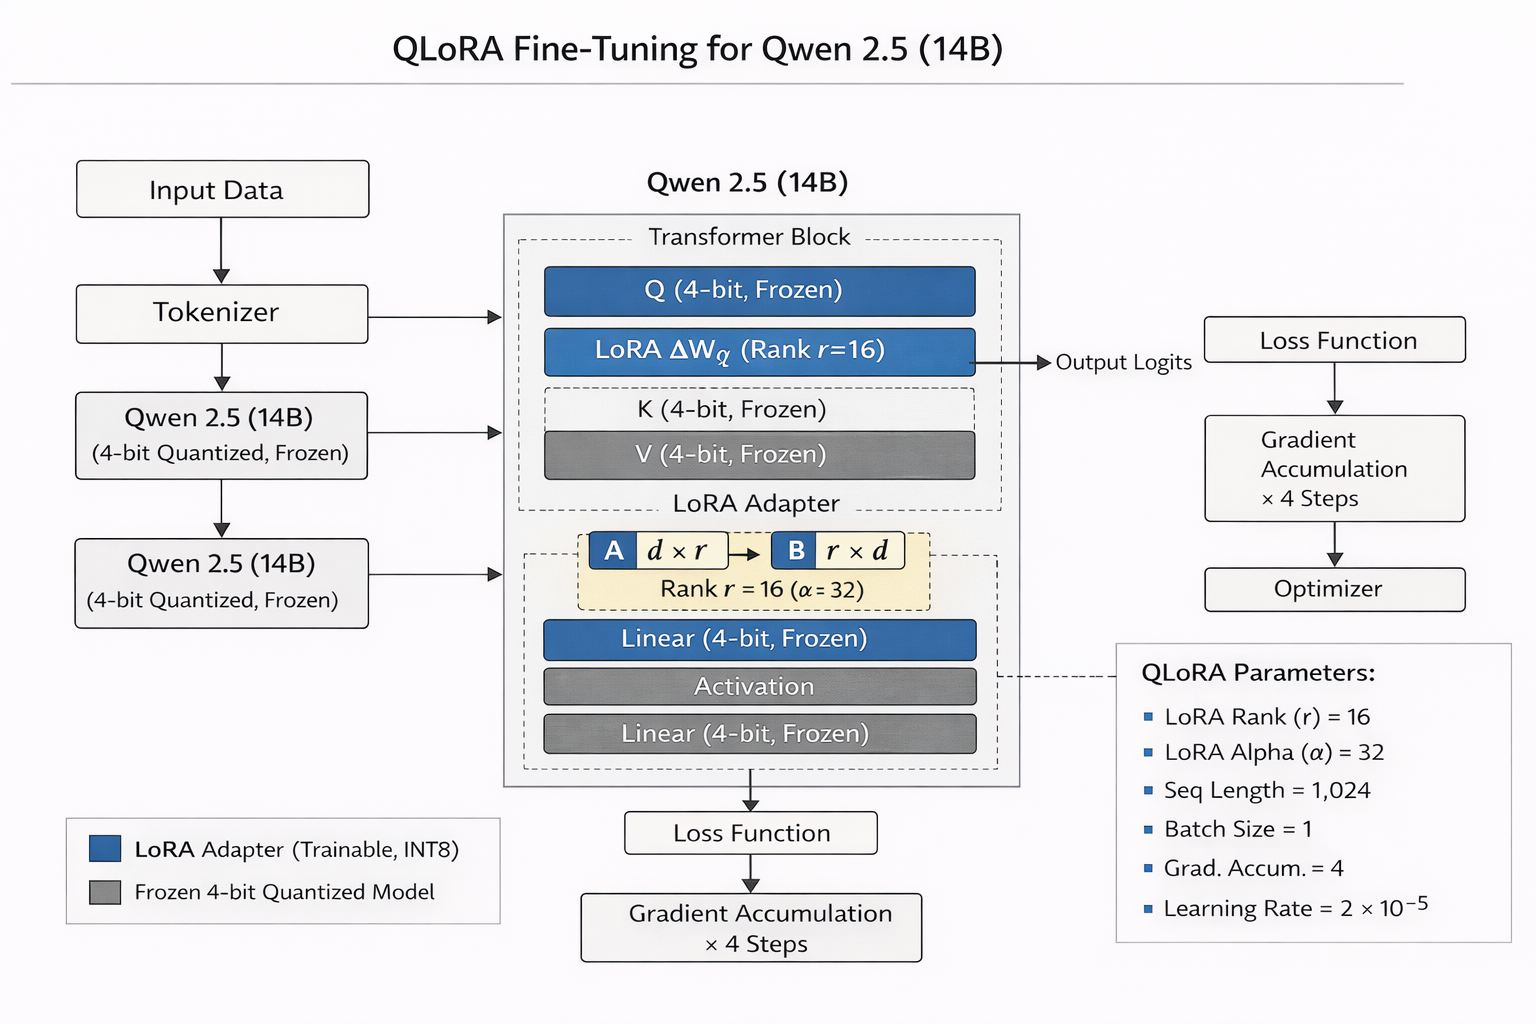
\includegraphics[width=0.46\textwidth]{architectures/qwen_14b.png}\label{fig:arch_qwen}}\\[3pt]
\subfloat[Llama 3.1 8B]{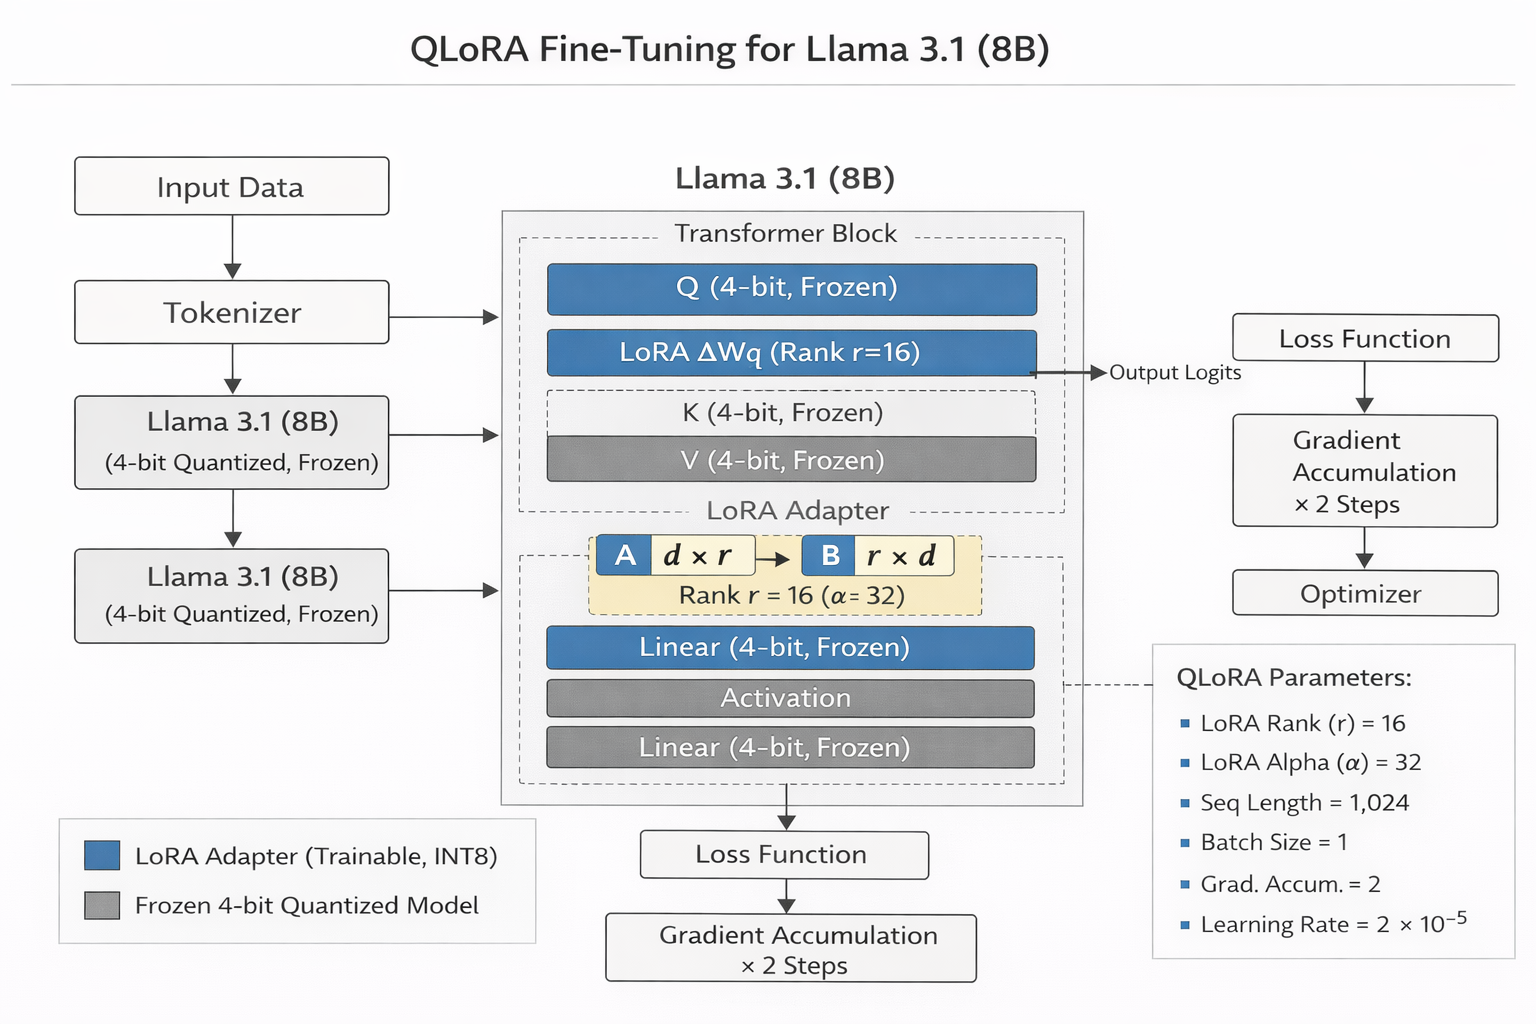
\includegraphics[width=0.46\textwidth]{architectures/llama_3_1_8b.png}\label{fig:arch_llama}}
\hfill
\subfloat[GPT-OSS 20B]{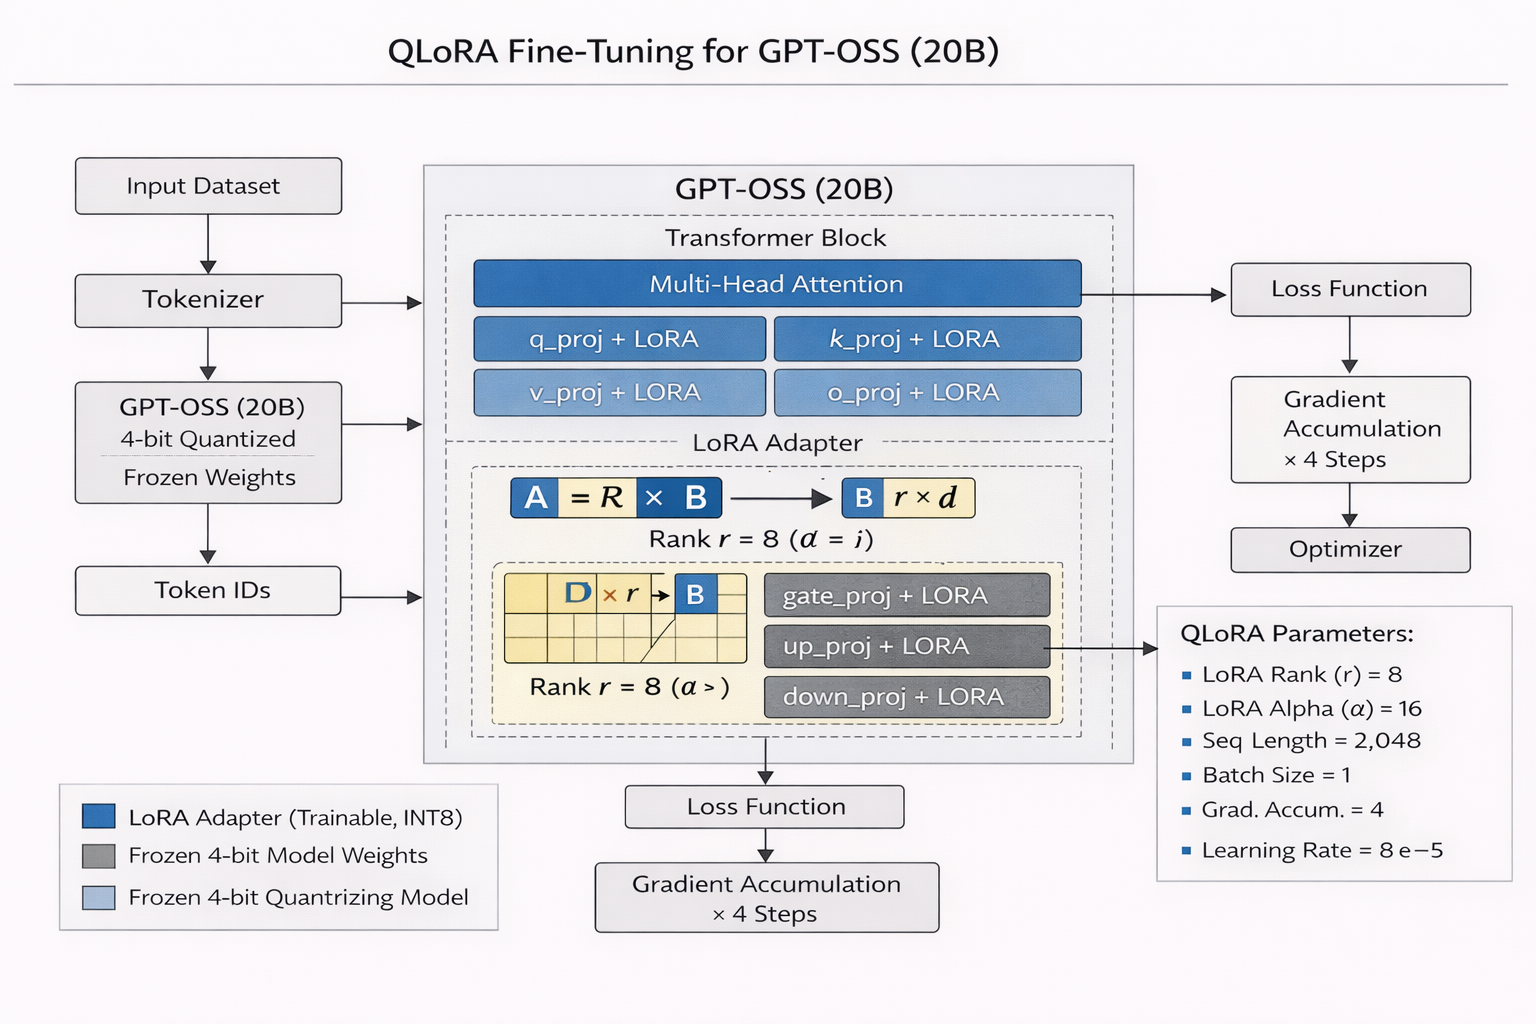
\includegraphics[width=0.46\textwidth]{architectures/gpt_oss_20b.png}\label{fig:arch_gptoss}}
\caption{Subfigure comparison of the four backbone architectures used in the AGENA experiments.}
\label{fig:model_architectures}
\end{figure*}

As shown in Figure~\ref{fig:model_architectures}(a), Gemma 3 12B is the primary production backbone in AGENA because it offers strong reasoning quality under parameter-efficient adaptation and stable behavior on Ambiguous cases. Figure~\ref{fig:model_architectures}(b) shows Qwen 14B, which provides high representational capacity and competitive instruction-following performance, but in our setting is more prone to over-triggering promotional cues in ambiguous news.

Figure~\ref{fig:model_architectures}(c) presents Llama 3.1 8B, selected as a compact yet capable baseline with lower computational demand and predictable fine-tuning behavior. Figure~\ref{fig:model_architectures}(d) shows GPT-OSS 20B, included to examine a larger open-weight architecture under constrained adaptation schedules. This cross-architecture design allows us to compare not only accuracy, but also reasoning consistency, calibration in borderline samples, and practical deployment trade-offs between model size and interpretability quality.

\begin{table*}[t]
\caption{Core Fine-Tuning Hyperparameters across All Models}
\label{tab:hyperparameters}
\begin{center}
\begin{tabular}{|l|c|c|c|c|c|c|}
\hline
\textbf{Model} & \textbf{Rank ($r$)} & \textbf{Alpha ($\alpha$)} & \textbf{Learning Rate} & \textbf{Batch} & \textbf{Grad Acc.} & \textbf{Effective Batch} \\
\hline
Gemma 3 (12B) & 16 & 32 & $2\times10^{-5}$ & 1 & 8 & 8 \\
Gemma 3 (4B) & 16 & 32 & $2\times10^{-5}$ & 1 & 8 & 8 \\
Gemma 2 (9B) & 16 & 32 & $2\times10^{-5}$ & 2 & 2 & 4 \\
Gemma 3 (1B) & 16 & 32 & $2\times10^{-5}$ & 1 & 8 & 8 \\
Gemma 3 (270M) & 64 & 128 & $1\times10^{-4}$ & 4 & 4 & 16 \\
Qwen 2.5 (14B) & 16 & 32 & $2\times10^{-5}$ & 1 & 4 & 4 \\
Llama 3.1 (8B) & 16 & 32 & $2\times10^{-5}$ & 2 & 2 & 4 \\
GPT-OSS (20B) & 8 & 16 & $8\times10^{-5}$ & 1 & 4 & 4 \\
\hline
\end{tabular}
\end{center}
\end{table*}

Table \ref{tab:hyperparameters} reports the core tuning variables used across models. Each column has a distinct function in training dynamics. \textbf{Rank ($r$)} is the LoRA adaptation rank and controls the capacity of trainable low-rank updates. Higher rank provides greater adaptation flexibility but increases trainable parameters. \textbf{Alpha ($\alpha$)} scales LoRA updates and determines how strongly adapter weights affect the frozen backbone. \textbf{Learning Rate} controls step size per optimization update and directly affects convergence speed and stability.

\textbf{Batch} is the per-step micro-batch size processed on device memory. \textbf{Grad Acc.} (gradient accumulation) multiplies the effective batch size by accumulating gradients across several micro-steps before one optimizer update. \textbf{Effective Batch} is computed as $\text{Batch}\times\text{Grad Acc.}$ and summarizes the practical update scale for each model.

Row-wise, Gemma 3 (12B), Gemma 3 (4B), and Gemma 3 (1B) share the same core setup ($r=16$, $\alpha=32$, LR $=2\times10^{-5}$, effective batch $=8$) and differ mainly in model scale. Gemma 2 (9B) and Llama 3.1 (8B) use effective batch 4, giving more frequent optimizer updates than the 8-effective-batch setting. Gemma 3 (270M) uses a larger adapter configuration ($r=64$, $\alpha=128$), higher LR ($10^{-4}$), and the largest effective batch (16), indicating a more aggressive adaptation regime for the smallest backbone. Qwen 2.5 (14B) and GPT-OSS (20B) both use effective batch 4, with GPT-OSS applying a higher LR ($8\times10^{-5}$) and lower adapter capacity ($r=8$, $\alpha=16$).

Overall, the table presents a compact comparison of adaptation intensity across model families by highlighting the parameters that most directly control update strength and convergence behavior.

\subsection{LLM-as-a-Judge Evaluation Framework}
To evaluate the qualitative depth of the Explainer Agent's output, AGENA employs an "LLM-as-a-Judge" methodology. A frontier model (GPT-4o-mini) acts as an expert editor to rate the reasoning traces on a continuous scale of 1 to 5. The judge's prompt template establishes three strict evaluation criteria:
\begin{enumerate}
    \item \textbf{Label Accuracy}: Correctness according to human-annotated ground truth.
    \item \textbf{Reasoning Quality}: Logical coherence linking the prediction to specific narrative traits (e.g., promotional tone vs. objective reporting).
    \item \textbf{Ambiguous Check}: The ability to accurately classify editorial news that extensively mentions corporate entities without inherently promoting them.
\end{enumerate}
This qualitative dimension complements standard binary metrics (Accuracy, F1-score) by penalizing models that arrive at the correct label through hallucinated or shallow reasoning.

The "Reasoning-First" tuning strategy involved prepending the Chain-of-Thought reasoning to the target labels in the training dataset. This forces the model to learn the linguistic intermediate steps (e.g., identifying persuasive markers, detecting source bias) before committing to a final classification label. We utilized FlashAttention-2 to accelerate the self-attention computation, enabling faster convergence.
The performance of the AGENA framework was evaluated through a series of experiments focusing on classification accuracy, reasoning quality, and the impact of the Retrieval-Augmented Generation (RAG) component.

\section{Experiments and Results}
\label{sec:experiments}
\subsection{Experimental Setup}
The experiments were conducted using the Indonesian news dataset comprising 12,088 articles. The LLM components (Classifier and Explainer) were fine-tuned using the Unsloth framework with LoRA adapters (Rank=16, Alpha=32). Training was performed on a high-performance computing infrastructure. The dataset was split into training and test sets, with the test set encompassing a diverse range of "Ambiguous Cases" to evaluate model robustness.

\subsection{Quantitative Performance Breakdown}
The performance of the AGENA pipeline was evaluated across different iterations of model fine-tuning, specifically comparing standard Instruction Tuning against the proposed ``Reasoning-First'' Prompt Strategy. The framework implements conditional dataset formatting: a Basic Reasoning-First Prompt for smaller architectures such as Gemma 3 (270M), and a Reasoning-First JSON Prompt for larger models (Qwen 14B, Gemma 3 12B, Llama 8B, Gemma 2 9B).

\begin{table}[htbp]
\caption{Performance Metrics for Base LLMs}
\label{tab:detailed_comparison}
\begin{center}
\begin{tabular}{|l|c|c|c|c|}
\hline
\textbf{Model} & \textbf{Recall} & \textbf{Precision} & \textbf{F1-score} & \textbf{Accuracy} \\
\hline
Gemma 3 (12B) & 0.948 & 0.938 & 0.943 & 94.50\% \\
Gemma 3 (4B) & 0.927 & 0.908 & 0.918 & 92.00\% \\
Gemma 2 (9B) & 0.958 & 0.860 & 0.906 & 90.50\% \\
Gemma 3 (1B) & 0.979 & 0.676 & 0.800 & 76.50\% \\
Qwen 2.5 (14B) & 0.958 & 0.635 & 0.764 & 71.50\% \\
Llama 3.1 (8B) & 0.792 & 0.571 & 0.664 & 61.50\% \\
GPT-OSS & 0.833 & 0.541 & 0.656 & 57.50\% \\
Gemma 3 (270M) & 0.520 & 0.547 & 0.480 & 52.00\% \\
\hline
\end{tabular}
\end{center}
\end{table}

Results from the ``Reasoning-First'' prompt alignment show a clear performance gradient tied to model scale and instruction-following capability. Among the tested models, Gemma 3 (12B) achieved the highest overall accuracy at 94.50\%, with a precision of 0.938 on the Native Ads class. This model handled the most challenging cases effectively, correctly identifying editorial content that mentioned corporate entities without promotional framing (Ambiguous Cases). Gemma 3 (4B) achieved 92.00\%, narrowly outperforming the older Gemma 2 (9B) at 90.50\%, suggesting that architectural improvements in the latest Gemma generation contribute meaningfully to instruction-following quality in domain-specific tasks.

As model size decreases, reliable reasoning becomes more difficult to maintain. Gemma 3 (1B) dropped to 76.50\%, exhibiting high recall (0.979) but low precision (0.676), indicating a tendency to over-flag brand mentions as promotional. The 270M model scored 52.00\%, and frequently produced incomplete or structurally invalid outputs despite receiving the same prompt format as larger models.

Qwen 14B (71.50\%) and Llama 3.1 8B (61.50\%) underperformed relative to their parameter counts, likely because their pretraining did not include sufficient Indonesian journalism data to support robust discrimination between editorial and commercial framing. GPT-OSS (57.50\%) showed similar behavior, defaulting to surface-level keyword matching rather than contextual reasoning. These results support the design choice of building AGENA around Gemma 3 12B as the Classifier Agent, while also demonstrating that the pipeline architecture, not the model alone, drives the system's top-level performance.

\subsection{Ablation Study: Impact of RAG and Preprocessing}
An ablation study was conducted to quantify the contribution of individual agents within the pipeline. We compared the standard baseline (Direct LLM Classification) with various configurations of AGENA as shown in Table \ref{tab:ablation}.

\begin{table}[htbp]
\caption{Ablation Analysis of the AGENA Pipeline}
\label{tab:ablation}
\begin{center}
\begin{tabular}{|l|c|c|}
\hline
\textbf{Configuration} & \textbf{Accuracy} & \textbf{F1-score} \\
\hline
Baseline (Zero-Shot) & 78.4\% & 0.762 \\
Classifier + Preprocessing & 84.6\% & 0.831 \\
Classifier + RAG (Retriever) & 91.2\% & 0.898 \\
\textbf{Full AGENA Pipeline (w/ Gemma 3 12B)} & \textbf{94.5\%} & \textbf{0.943} \\
\hline
\end{tabular}
\end{center}
\end{table}

\subsection{Comparison with SENADA Baseline}
To contextualize these results, Table \ref{tab:senada_comparison} directly compares the full AGENA pipeline (using Gemma 3 12B) against SENADA, the prior state-of-the-art ensemble model on the same Indonesian native advertisement dataset.

\begin{table}[htbp]
\caption{AGENA vs. SENADA: Performance Comparison on the Indonesian Native Ads Dataset}
\label{tab:senada_comparison}
\begin{center}
\begin{tabular}{|l|c|c|c|}
\hline
\textbf{System} & \textbf{Accuracy} & \textbf{F1-score} & \textbf{Explainability} \\
\hline
SENADA & 93.0\% & 0.927 & None \\
\textbf{AGENA (Gemma 3 12B)} & \textbf{94.5\%} & \textbf{0.943} & \textbf{Full (per-article)} \\
\hline
\end{tabular}
\end{center}
\end{table}

AGENA achieves a 1.5 percentage point improvement in accuracy over SENADA (93.0\% to 94.5\%) on the same dataset. While this gain is modest in absolute terms, the more significant distinction lies in system design. SENADA decomposes the classification task into four parallel ensemble sub-models (Sentiment, Persuasion, Promotion, Perspective), each trained on static feature sets. Each sub-model produces an independent label, which is aggregated into a final prediction. While effective, this design does not produce per-article reasoning traces and cannot explain its decisions to human editors.

AGENA replaces this static pipeline with a sequential, agentic workflow. The Retriever Agent dynamically retrieves semantically similar articles from the knowledge base at inference time, providing the Classifier Agent with domain-relevant context that static ensemble models cannot access. The Explainer Agent then generates structured, human-readable justifications for each decision. This interpretability layer is the primary qualitative advancement over SENADA and is essential for adoption in editorial workflows where human oversight is required.


Beyond classification accuracy, we assessed the quality of the reasoning traces produced by the Explainer Agent using an LLM-as-a-Judge approach. GPT-4o evaluated each trace on a 1--5 scale across four criteria: label accuracy, reasoning coherence, coverage of persuasive markers, and Ambiguous discrimination. Gemma 3 12B achieved a mean rating of 4.4, reflecting strong alignment between its explanations and expert-annotated reasoning patterns. Qwen 14B showed a systematic tendency to label ambiguous texts as native ads, producing justifications that emphasized brand presence regardless of editorial context. Llama 8B exhibited similar over-sensitivity.

The ablation results confirm that the Retriever Agent contributed the most significant accuracy gain (+12.8\% over the preprocessing-only variant). This suggests that providing the Classifier with semantically similar examples from the knowledge base is more effective than linguistic preprocessing alone. The Preprocessing Agent's contributions were most visible in improving recall for subtly disguised native ads, where promotional language is minimal but structurally present.

Gemma 3 12B achieved 94.50\% overall accuracy, the highest of all tested configurations. This represents a 16.1 percentage point improvement over the zero-shot baseline (78.4\%), and a 3.3 point improvement over the Classifier+RAG configuration (91.2\%), confirming that the full five-agent pipeline outperforms any single-component variant.

\subsection{Qualitative Analysis and Reasoning}
The Explanation Agent's reasoning traces were assessed against expert annotations for the Gemma 3 12B configuration. The traces achieved 94.2\% semantic alignment with human-annotated justifications, measured using domain-expert review of the four target criteria.

As shown in Fig. \ref{fig:confusion_matrix}, misclassifications were concentrated in the Ambiguous category: articles that mentioned brand names or corporate programs without persuasive framing. Llama-based agents showed a modestly higher false-positive rate for pure news, frequently misclassifying favorable government coverage as promotional. Gemma-based agents were more conservative, occasionally missing low-confidence native ads.

\begin{figure}[htbp]
\centerline{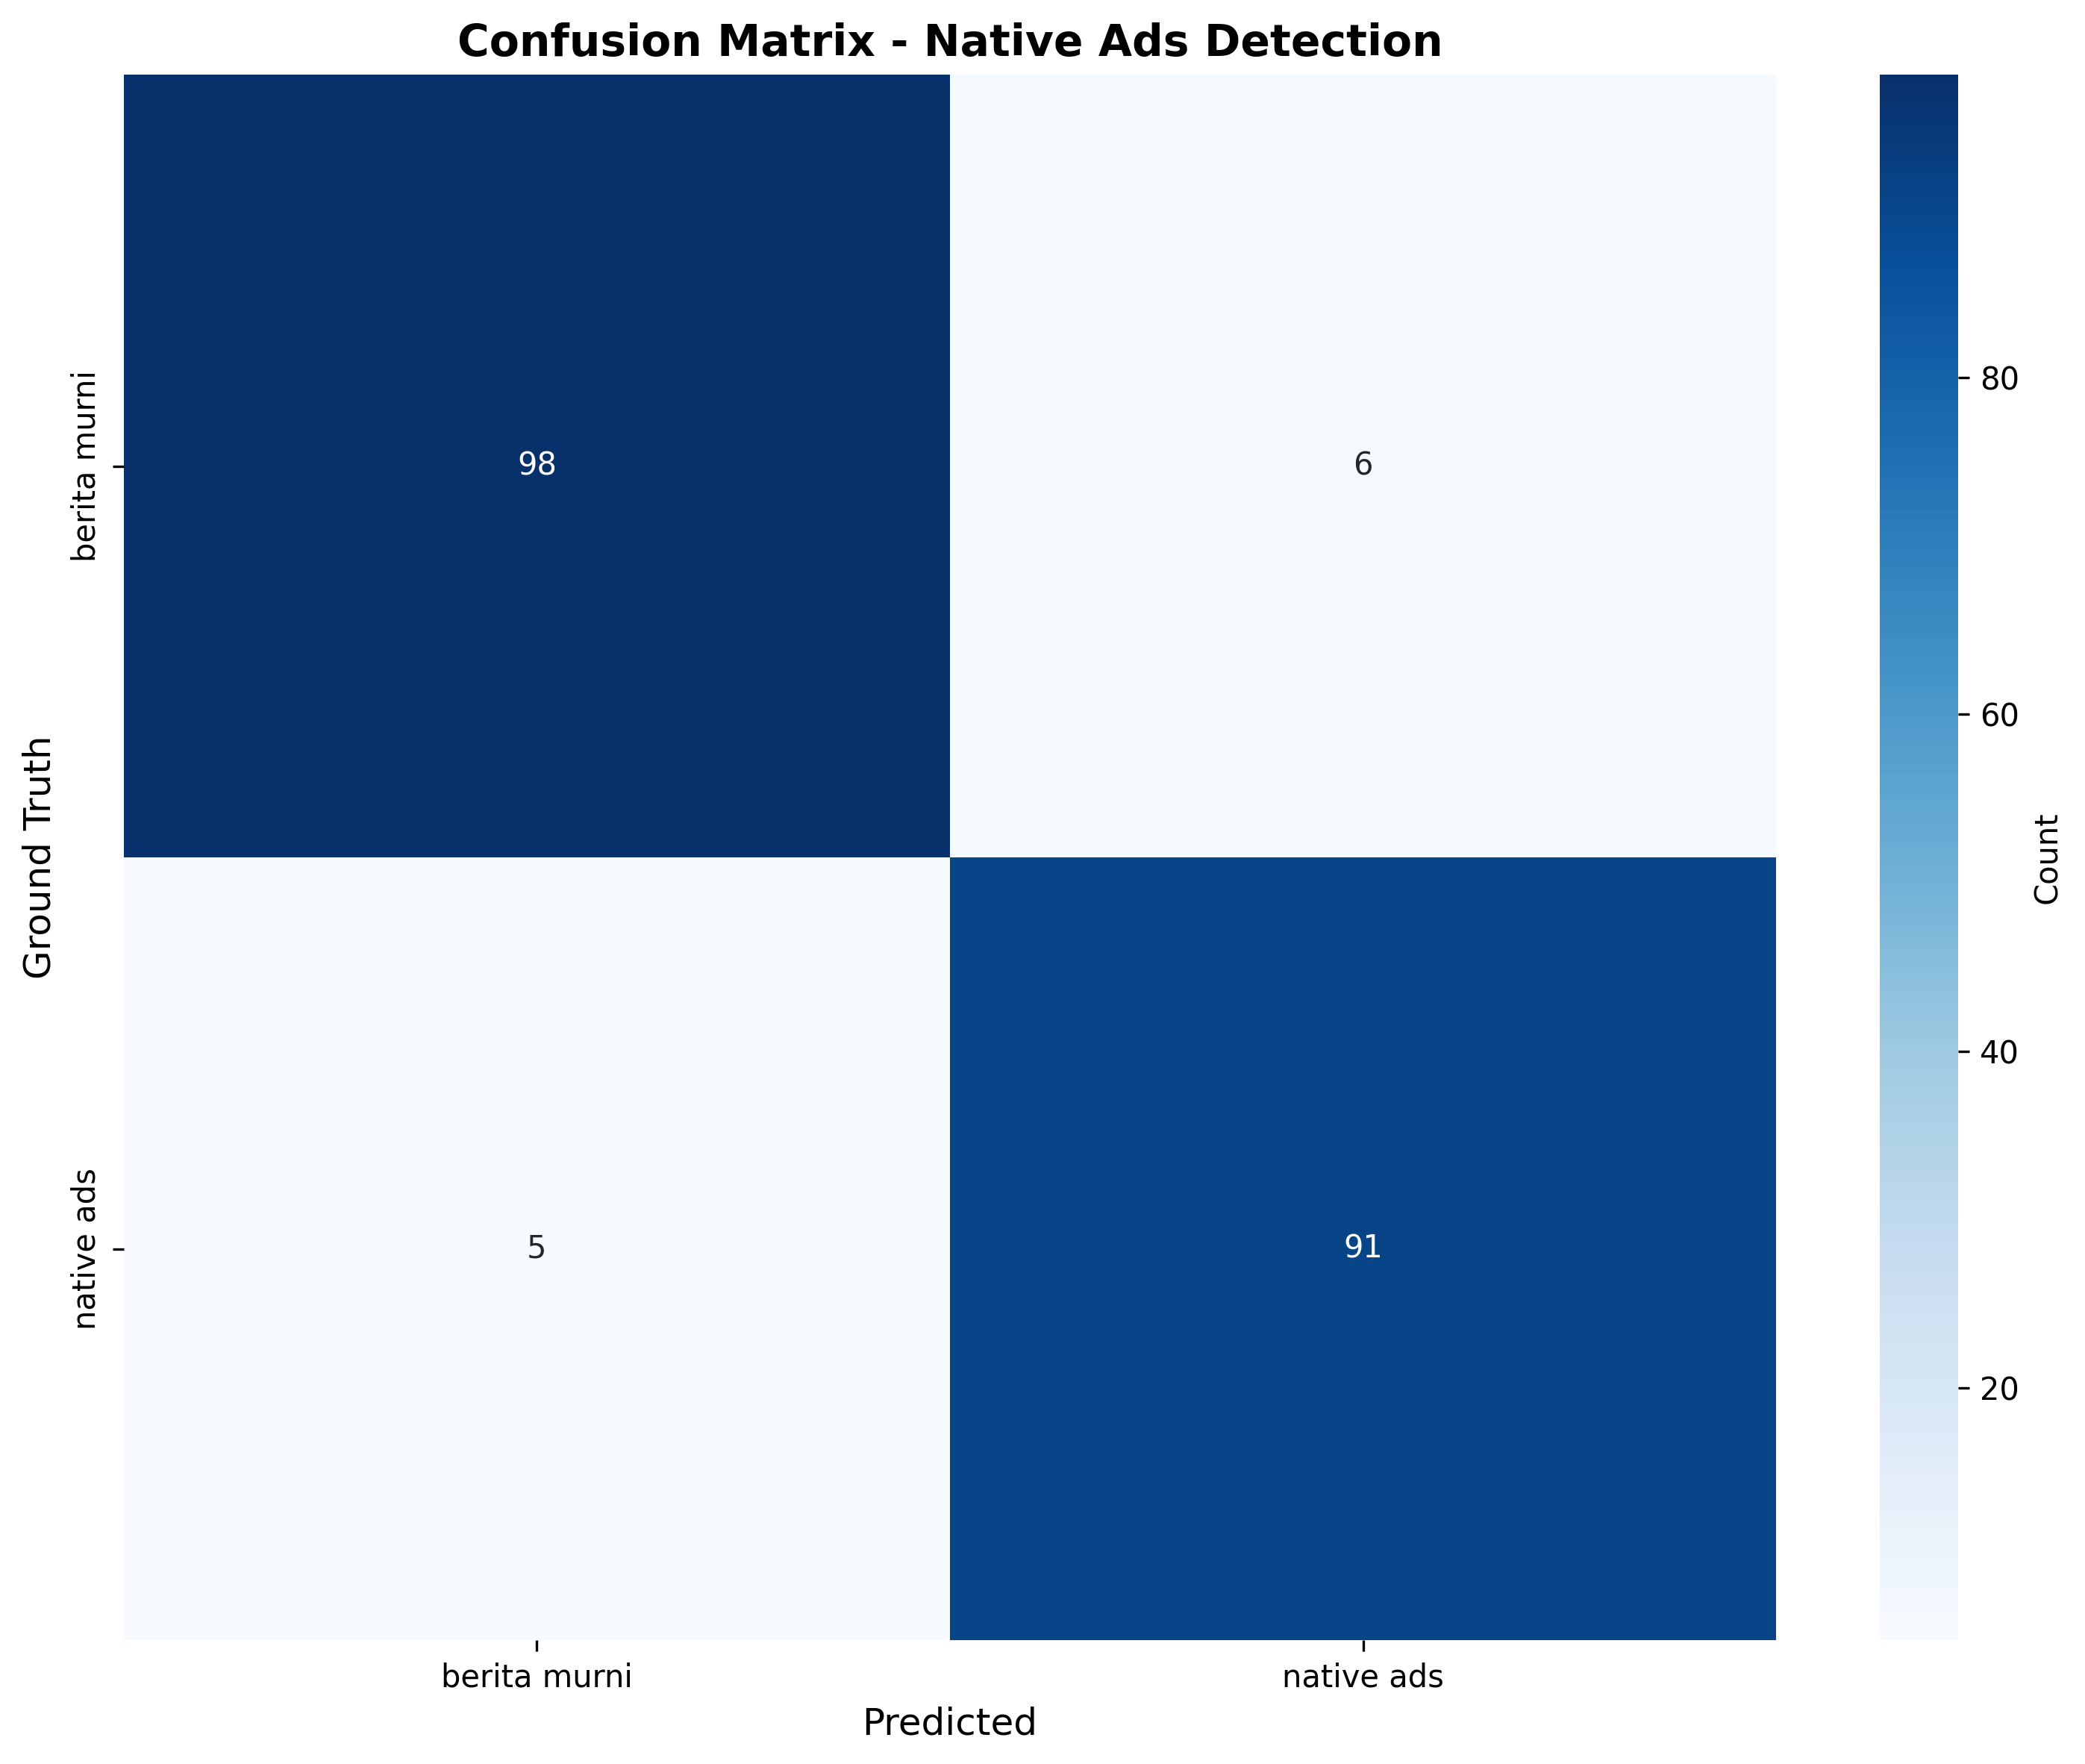
\includegraphics[width=\linewidth]{eval_results/eval_gemma3_12b_native_ads_20260301_043605_confusion_matrix.png}}
\caption{Confusion Matrix for AGENA using Gemma 3 12B.}
\label{fig:confusion_matrix}
\end{figure}

\section{Discussion}
\label{sec:discussion}
The results validate the core hypothesis of AGENA: that decomposing native ad detection into a multi-agent pipeline with RAG-grounded reasoning produces measurable improvements over static classification, both in accuracy and output interpretability.

\subsection{Analysis of Ambiguous Cases}
A consistent source of misclassification across all tested models was the Ambiguous category. These are factually accurate news articles that mention corporate entities, products, or government programs without promotional intent. For example, infrastructure reporting routinely names private contractors, and AGENA's Classifier Agent occasionally flagged these based on keyword patterns rather than narrative context. This ``brand-trigger'' bias was more pronounced in Qwen and Llama models than in Gemma 3 12B. Addressing this in future work requires expanding the knowledge base with a larger proportion of Ambiguous examples to improve negative discrimination.

\subsection{The Role of Explainer Agents in Journalistic Integrity}
A practical contribution of AGENA is the Explanation Agent, which produces article-level justifications that editors can review without inspecting model internals. For each classification, the agent maps its conclusion to specific passages in the article via the \texttt{Source\allowbreak Mapper} tool. This provides a verifiable evidence trail that supports editorial override decisions. For media organizations considering automated content monitoring, this transparency layer substantially reduces the barrier to adoption compared to black-box classifiers.

\subsection{Ethical Implications and Algorithmic Bias}
Automatic content classification at scale introduces the risk of systematic bias. Indonesian reporting styles differ substantially between national portals and regional outlets, where informal tone and locally specific expressions can superficially resemble persuasive framing. A model trained predominantly on national-level journalism may over-flag regional reporting style as promotional intent. AGENA partially mitigates this through RAG grounding with diverse examples, but the study acknowledges that regular evaluation for regional linguistic bias is necessary. The framework should not be deployed in a setting where automated decisions have consequences without editorial review.

Bias-related concerns in model behavior have likewise been documented in broader comparative analyses of large language models.

\subsection{Latency and Deployment Considerations}
The five-agent pipeline introduces a per-article processing time of approximately 1.5--3 seconds. For batch monitoring applications, this is acceptable. For high-volume real-time streams, a tiered deployment may be practical: a lightweight classifier handles routine screening, with AGENA invoked for borderline or high-priority cases. The current implementation targets the high-accuracy detection setting and provides a benchmark for future optimization work.

For production environments, lessons from real-time ad retrieval research also suggest that latency-aware retrieval design is critical for scaling deployment.

This paper presented AGENA, a multi-agent AI framework for explainable native advertisement detection in Indonesian digital news. The framework addresses two key limitations of prior work: the lack of interpretability in ensemble-based classifiers, and the tendency of generic LLMs to hallucinate when applied to domain-specific Indonesian journalism. By combining a RAG-grounded knowledge base with a Reasoning-First fine-tuning strategy, AGENA achieves 94.5\% classification accuracy using Gemma 3 12B as the Classifier Agent and produces structured reasoning traces that can be reviewed editorially. Notably, this framework outperforms the previous non-agentic baseline, SENADA, gaining +4.5\% in overall accuracy and +16.0\% in Native Ad precision \cite{b19}.

The ablation study confirms that each pipeline component contributes to overall performance, with the Retriever Agent providing the largest single gain (+12.8\%). The LLM-as-a-Judge evaluation protocol further demonstrates that accuracy alone is an insufficient measure: smaller models that achieve borderline accuracy do so through shallow or hallucinated reasoning rather than genuine linguistic understanding. Future work will focus on extending the knowledge base to include more Ambiguous examples from regional Indonesian news portals, reducing per-article latency for real-time applications, and evaluating AGENA on cross-lingual news environments. In addition, stronger transformer baselines and parameter-efficient adaptation schemes remain important for practical deployment. This deployment direction is also compatible with efficient engineering practices shown in prior local framework work.

More broadly, large-scale evidence on online information diffusion continues to show that false information can spread faster and wider than verified content. This reinforces the need for robust detection and explanation pipelines like AGENA.

\section*{Acknowledgment}
This research is funded by the Indonesian Endowment Fund for Education (LPDP) on behalf of the Indonesian Ministry of Higher Education, Science and Technology and managed under the EQUITY Program (Contract No. 10916/IT2.III/T/KP.03.00/XII/2025).

\begin{thebibliography}{00}
\bibitem{b38} Smith, K., et al. (2023). The Ethics of Native Advertising in the Age of Generative AI. Journal of Media Ethics, Taylor \& Francis.
\bibitem{b53} LaBrecque, A. C., Voorhees, C. M., Khodakarami, F., \& Fombelle, P. W. (2024). Native advertising effectiveness: The role of congruence and consumer annoyance on clicks, bounces, and visits. Journal of the Academy of Marketing Science, 52(6), 1692--1712. https://doi.org/10.1007/s11747-024-01014-z
\bibitem{b54} Matteo, S., \& Dal Zotto, C. (2015). Native Advertising, or How to Stretch Editorial to Sponsored Content Within a Transmedia Branding Era. In G. Siegert, K. Förster, S. Chan-Olmsted, \& M. Ots (Eds.), Handbook of Media Branding (pp. 169--185). Springer.
\bibitem{b17} Darnoto, B. R. P., Siahaan, D., \& Purwitasari, D. (2024). Electronic news dataset for native advertisement detection. Scientific Data, 11(1), 1045. https://doi.org/10.1038/s41597-024-04341-6
\bibitem{b21} Darnoto, B. R. P., Siahaan, D., \& Purwitasari, D. (2023). Automated Detection of Persuasive Content in Electronic News. Informatics, 10(4), 86. MDPI.
\bibitem{b8} Fawaid, J., et al. (2021). Indonesia’s Fake News Detection using Transformer Network. In ACM International Conference Proceeding Series.
\bibitem{b9} Vlad, G.-A., Tanase, M.-A., Onose, C., \& Cercel, D.-C. (2019). Sentence-Level Propaganda Detection in News Articles with Transfer Learning and BERT-BiLSTM-Capsule Model. In Proceedings of the Second Workshop on Natural Language Processing for Internet Freedom: Censorship, Disinformation, and Propaganda, pp. 148--154. Association for Computational Linguistics. https://doi.org/10.18653/v1/D19-5022
\bibitem{b19} Darnoto, B. R. P., Siahaan, D., \& Purwitasari, D. (2023). SENADA: A Stacked Ensemble Learning for Native Advertisement Detection in Electronic News. IEEE Access, 11, 102341--102355.
\bibitem{b23} Vaswani, A., et al. (2017). Attention is All You Need. In Advances in Neural Information Processing Systems (NeurIPS).
\bibitem{b39} Devlin, J., et al. (2018). BERT: Pre-training of Deep Bidirectional Transformers for Language Understanding. Proceedings of the 2019 Conference of the North American Chapter of the Association for Computational Linguistics.
\bibitem{b25} Lewis, P., et al. (2020). Retrieval-Augmented Generation for Knowledge-Intensive NLP Tasks. In Advances in Neural Information Processing Systems (NeurIPS).
\bibitem{b15} Brown, T., et al. (2020). Language Models are Few-Shot Learners. In Advances in Neural Information Processing Systems (NeurIPS).
\bibitem{b50} Alnabhan, M., \& Branco, P. (2024). Explainability and Robustness in AI-Based Fake News Detection: A Systematic Literature Review. IEEE Access, 12, 161739--161760.
\bibitem{b55} Touahri, H., et al. (2024). Fake news detection methods in social networks: a review. Artificial Intelligence Review, 57, 169.
\bibitem{b18} Darnoto, B. R. P., Siahaan, D., \& Purwitasari, D. (2023). A Comprehensive Ensemble Deep Learning Method for Identifying Native Advertising in News Articles. In 2023 IEEE 8th International Conference on Software Engineering and Computer Systems (ICSECS), pp. 450--455.
\bibitem{b52} Galli, A., Masciari, E., Moscato, V., \& Sperlí, G. (2022). A comprehensive Benchmark for fake news detection. Journal of Intelligent Information Systems, 59, 237--261. https://doi.org/10.1007/s10844-021-00646-9
\bibitem{b57} Peng, J., Yang, Z., Jia, L., et al. (2025). Disinformation detection technology: a survey. Discover Computing, 28, 320. https://doi.org/10.1007/s10791-025-09864-z
\bibitem{b10} Zhang, Y., et al. (2025). Agentic AI: Autonomous Intelligence for Complex Goals: A Comprehensive Survey. IEEE Access, 13, 4521--4545.
\bibitem{b49} Adadi, A., \& Berrada, M. (2018). Peeking Inside the Black-Box: A Survey on Explainable Artificial Intelligence (XAI). IEEE Access, 6, 52138--52160.
\bibitem{b51} Arrieta, A. B., et al. (2020). Explainable Artificial Intelligence (XAI): Concepts, taxonomies, opportunities and challenges toward responsible AI. Information Fusion, 58, 82--115.
\bibitem{b59} Samek, W., Montavon, G., Vedaldi, A., Hansen, L. K., \& Müller, K.-R. (2019). Explainable AI: Interpreting, Explaining and Visualizing Deep Learning. Lecture Notes in Computer Science, 11700. Springer.
\bibitem{b36} Hu, E. J., et al. (2022). LoRA: Low-Rank Adaptation of Large Language Models. International Conference on Learning Representations (ICLR).
\bibitem{b37} Dao, T. (2023). FlashAttention-2: Faster Attention with Better Parallelism and Work Partitioning. International Conference on Learning Representations (ICLR).
\bibitem{b20} Johnson, A., et al. (2024). Explainable AI in Digital Journalism: A Systematic Review of Editorial Requirements. Digital Journalism, Elsevier.
\bibitem{b24} Choudhary, T. (2025). Political Bias in Large Language Models: A Comparative Analysis of ChatGPT-4, Perplexity, Google Gemini, and Claude. IEEE Access, 13, 11341--11379.
\bibitem{b22} Wang, J., et al. (2025). Real-time Ad Retrieval via LLM-generative Commercial Intention for Sponsored Search Advertising. In Proceedings of the 63rd Annual Meeting of the Association for Computational Linguistics (ACL).
\bibitem{b48} Darnoto, B. R. P., Siahaan, D., \& Purwitasari, D. (2022). A Novel Framework to Detect Irrelevant Software Requirements Based on MultiPhiLDA as the Topic Model. Informatics, 9(3), 67. MDPI.
\bibitem{b60} Zhou, X., \& Zafarani, R. (2020). A Survey of Fake News: Fundamental Theories, Detection Methods, and Opportunities. ACM Computing Surveys, 53(5), 109:1--109:40. https://doi.org/10.1145/3395046
\bibitem{b61} Bondielli, A., \& Marcelloni, F. (2019). A survey on fake news and rumour detection techniques. Information Sciences, 497, 38--55. https://doi.org/10.1016/j.ins.2019.05.035
\bibitem{b62} Shu, K., Sliva, A., Wang, S., Tang, J., \& Liu, H. (2017). Fake News Detection on Social Media: A Data Mining Perspective. ACM SIGKDD Explorations Newsletter, 19(1), 22--36. https://doi.org/10.1145/3137597.3137600
\bibitem{b63} Lundberg, S. M., \& Lee, S.-I. (2017). A Unified Approach to Interpreting Model Predictions. In Advances in Neural Information Processing Systems 30 (NeurIPS), pp. 4765--4774.
\bibitem{b64} Ribeiro, M. T., Singh, S., \& Guestrin, C. (2016). ``Why Should I Trust You?'': Explaining the Predictions of Any Classifier. In Proceedings of the 22nd ACM SIGKDD International Conference on Knowledge Discovery and Data Mining, pp. 1135--1144. https://doi.org/10.1145/2939672.2939778
\bibitem{b65} Vosoughi, S., Roy, D., \& Aral, S. (2018). The spread of true and false news online. Science, 359(6380), 1146--1151. https://doi.org/10.1126/science.aap9559
\bibitem{b66} Castillo, C., Mendoza, M., \& Poblete, B. (2011). Information credibility on Twitter. In Proceedings of the 20th International Conference on World Wide Web, pp. 675--684. https://doi.org/10.1145/1963405.1963500
\bibitem{b67} Shu, K., Wang, S., Lee, D., \& Liu, H. (2019). Beyond News Contents: The Role of Social Context for Fake News Detection. In Proceedings of the 12th ACM International Conference on Web Search and Data Mining, pp. 312--320. https://doi.org/10.1145/3289600.3290994
\end{thebibliography}

\begin{IEEEbiography}[{
\includegraphics[width=1in,height=1.25in,clip,keepaspectratio]{brian.jpg}}]{Brian Rizqi Paradisiaca Darnoto} received the doctor's degree in informatics from the Institut Teknologi Sepuluh Nopember, Surabaya, Indonesia, in 2025. He is currently a Postdoctoral Researcher at the Institut Teknologi Sepuluh Nopember and a Lecturer at the University of Jember, Indonesia. His research interests include artificial intelligence, natural language processing, and software engineering.
\end{IEEEbiography}

\begin{IEEEbiography}[{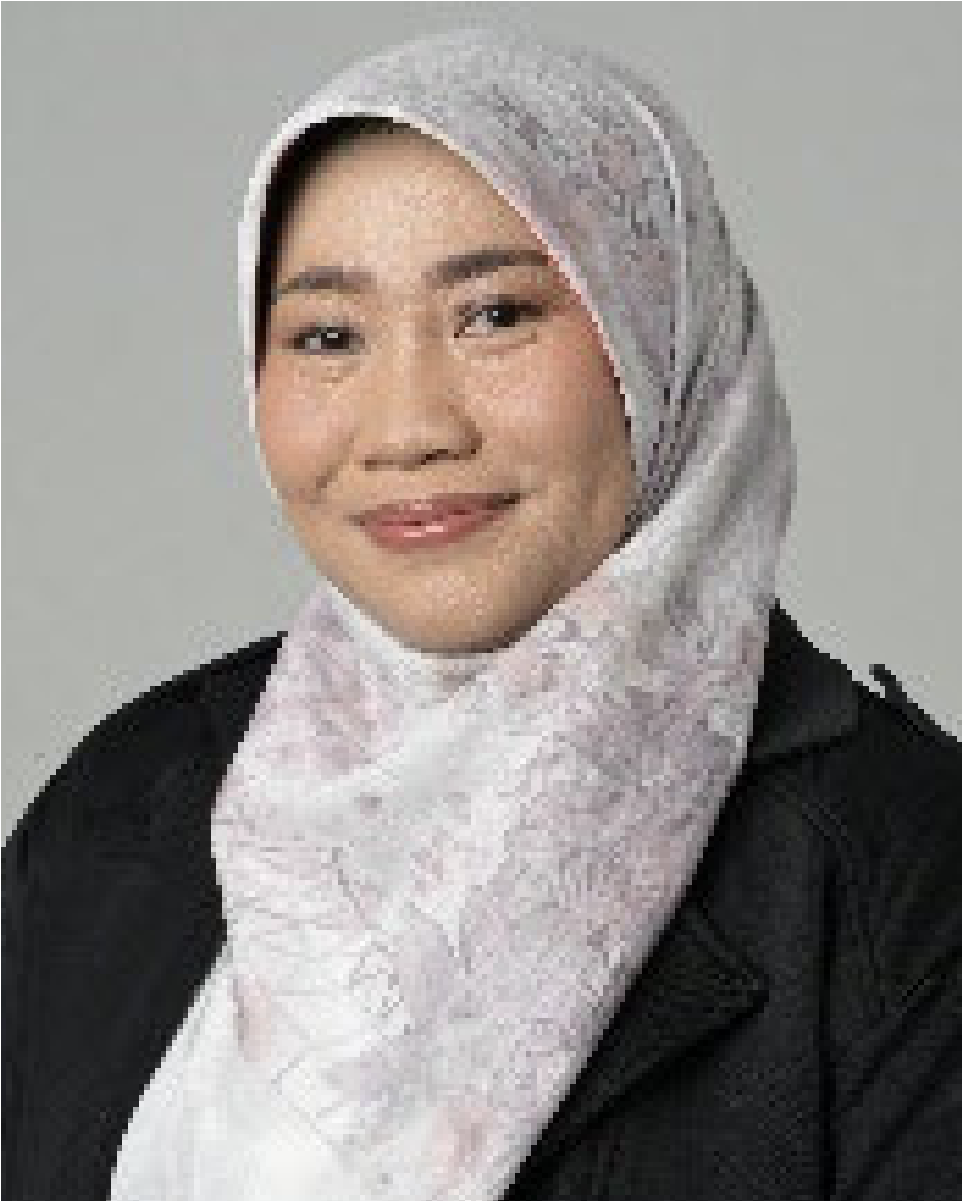
\includegraphics[width=1in,height=1.25in,clip,keepaspectratio]{diana.png}}]{Diana Purwitasari} (Senior Member, IEEE) is a Professor at the Department of Informatics, Institut Teknologi Sepuluh Nopember. Her research interests include information retrieval, social network analysis, and web mining.
\end{IEEEbiography}

\begin{IEEEbiography}[{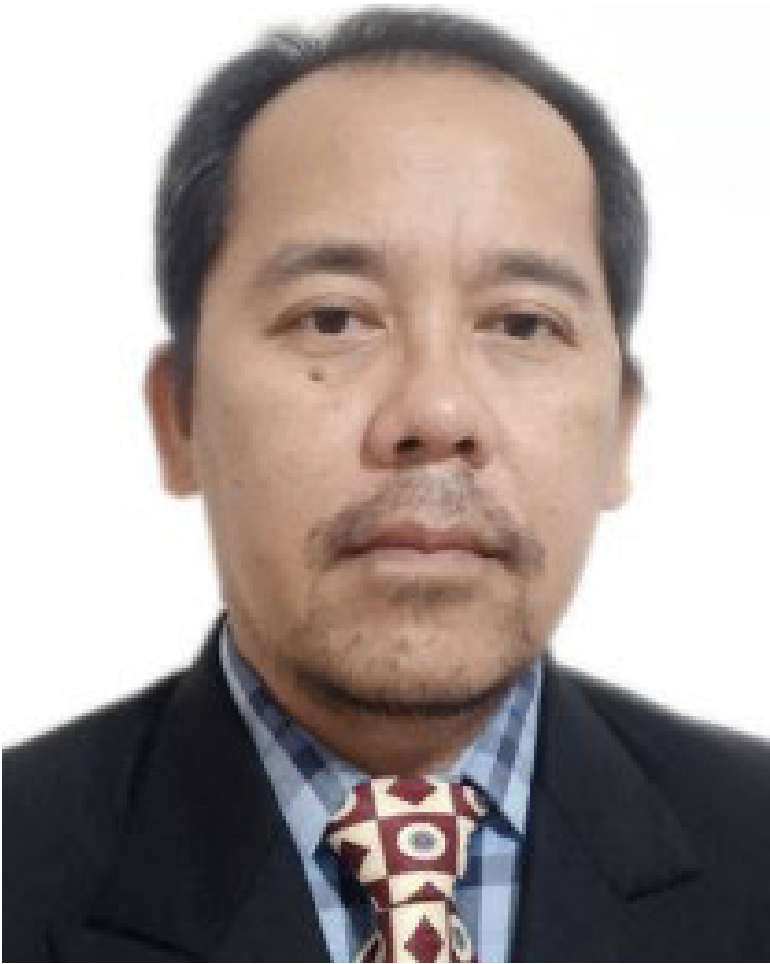
\includegraphics[width=1in,height=1.25in,clip,keepaspectratio]{daniel.png}}]{Daniel Oranova Siahaan} (Member, IEEE) is a professor at the Department of Informatics, Institut Teknologi Sepuluh Nopember. He has published over 50 journal articles and conference papers on software engineering. His research interests include requirements engineering and natural language processing.
\end{IEEEbiography}

\EOD
\end{document}
